\section{Indução eletromagnética}

\frame{
	\frametitle{Indução eletromagnética}
	\begin{block}{Introdução}
		Em 1820, Hans Christian Oersted descobriu que a passagem de uma corrente elétrica em um condutor mudava a direção da agulha de uma bússola. Ou seja, ele descobriu o \textbf{eletromagnetismo}.
		\begin{itemize}
			\item A partir daí, muitos cientistas começaram a investigar mais profundamente a conexão entre os fenômenos elétricos e magnéticos. Eles buscavam, principalmente, descobrir se o efeito contrário era possível, isto é, se \textbf{os efeitos magnéticos poderiam gerar uma corrente elétrica}.
		\end{itemize}
	\end{block}
}

\frame{
	\frametitle{Indução eletromagnética}
	\begin{block}{Descoberta}
		Assim, em 1831, \textbf{Michael Faraday} com base em resultados experimentais, descobriu o fenômeno da \textbf{indução eletromagnética}.
		\begin{itemize}
			\item A \textbf{Lei de Faraday} e a \textbf{Lei de Lenz} são duas leis fundamentais do eletromagnetismo e determinam a \textbf{indução eletromagnética}.
		\end{itemize}
	\end{block}
}

\frame{
	\frametitle{Indução eletromagnética}
	\begin{block}{Definição}
		Indução eletromagnética é o fenômeno relacionado ao \textbf{aparecimento de uma corrente elétrica} em um condutor imerso em um campo magnético, \textbf{quando ocorre variação do fluxo} que o atravessa.
	\end{block}
}

\frame{
	\frametitle{Indução eletromagnética}
	\begin{block}{Definição}
		Podemos dizer que com uma simples movimentação de um ímã próximo a uma espira é possível produzir corrente elétrica. A produção de corrente elétrica por campos magnéticos recebeu o nome de \textbf{indução eletromagnética} e a corrente gerada por meio desse processo é chamada de \textbf{corrente induzida}.
	\end{block}

	\centering
	\setmyunit{1.5cm}
	\begin{tikzpicture}[scale=0.5]
			\draw (-4,-3) rectangle (4,3); %CLP
		\draw (-4,0) -- (-2.5,0); %Div in out
		\draw (-2.5,-3) -- (-2.5,3); %Div cartoes
		\draw (-1.5,-2.5) rectangle (0,2.5); %Mem dados
		\draw (0.5,-2.5) rectangle (3.5,-1); %Mem prog
		\draw (1,0) rectangle (3,2); %CPU
		\draw (-4,-5) rectangle (4,-3); %Alimentacao
		\draw (-2.5,4) rectangle (4,6); %Term de prog
		
		\draw (1,2.6) node {CLP};
		
		\draw (-3.25,1.5) node[text width=1.5cm,align=center,rotate=90] {\small Cartões de input};
		
		\draw (-3.25,-1.5) node[text width=1.5cm,align=center,rotate=90] {\small Cartões de output};
		
		\node at (2,1) {\small CPU};
		
		\node[rotate=90,text width=1.5cm,align=center] at (-0.75,0) {\small Memória de dados};
		
		\node[text width=2cm,align=center] at (2,-1.75) {\footnotesize Memória de programa};
		
		\node at (-6,0) {Campo};
		
		\node at (0,-4) {Alimentação};
		
		\node[text width=3cm,align=center] at (0.75,5) {Terminal de programação};
		
		\draw[-Latex] (-8,1.5) -- node[above] {Entradas} +(4,0);
		\draw[Latex-] (-8,-1.5) -- node[below] {Saídas} +(4,0);
		\draw[-Latex] (-2.5,1.5) -- +(1,0);
		\draw[Latex-] (-2.5,-1.5) -- +(1,0);
		\draw[-Latex] (0,1.5) -- +(1,0);
		\draw[Latex-] (0,0.5) -- +(1,0);
		\draw[Latex-] (2,0) -- +(0,-1);
		
		\draw[-Latex] (-1.5,4) -- +(0,-1);
		\draw[Latex-] (3,4) -- +(0,-1);
	\end{tikzpicture}
%	\centerline{\includegraphics[width=0.6\linewidth]{Figuras/Ch10/fig1.jpg}}
}

\frame{
	\frametitle{Fluxo magnético}
	\begin{block}{Introdução}
		Para que se entenda o que é, e como se origina a indução eletromagnética é necessário que definamos uma grandeza física chamada \textbf{fluxo magnético}. Esta grandeza é vetorial é simbolizada por $\vec{\Phi}$.
	\end{block}
}

\frame{
	\frametitle{Fluxo magnético}
	\begin{block}{Definição}
		Podemos escrever o fluxo magnético como o produto do vetor indução magnética (campo magnético) $\vec{B}$ pela área da superfície $A$ e pelo cosseno do ângulo $\theta$, formado entre e uma linha perpendicular à superfície, chamada reta normal.
		$$\boxed{\vec{\Phi} = B \cdot A \cdot \cos \theta}$$
		\begin{itemize}
			\item A unidade adotada para se medir o fluxo de indução magnética pelo SI é o \textbf{Weber} (Wb), em homenagem ao físico alemão Wilhelm Webber, e caracteriza Tesla por metro quadrado (T/m$^2$).
		\end{itemize}
	\end{block}
}

\frame{
	\frametitle{Fluxo magnético}
	\begin{block}{Definição}
		\begin{itemize}
			\item É possível também se associar o fluxo de indução magnética à \textbf{quantidade de linhas de indução que atravessam a superfície}.
		\end{itemize}
	\end{block}
%	\vspace{0.5cm}

	\centering
	
	\setmyunit{1cm}
	\begin{tikzpicture}
	\foreach \x in {-1.5,-1,...,1.5}
	\draw[blue] (0,\x) -- +(2,0);
	
	\draw (5.5,0) node[blue] {$ \vec{B} $};
	
	\filldraw[fill=black!40!white,draw=black,rotate=-30] (2,1) circle (1.5 and 0.5);
	
	\foreach \x in {-1.5,-1,1,1.5}
	\draw[-Latex,blue] (2,\x) -- +(3,0);
	
	\draw[-Latex,blue] (1.5,0.5) -- (5,0.5);
	\draw[-Latex,blue,name path=midb] (2.2,0) -- (5,0);
	\draw[-Latex,blue] (2.8,-0.5) -- (5,-0.5);
	
	\draw[rotate=-30] (2,1) rectangle +(0.1,0.1) node[pos=.5] {$ \cdot $};
	\draw[-Latex,rotate=-30,name path=nar] (2,1) -- node[above,rotate=60] {Reta normal} +(0,2) node[name=B,coordinate] {};
	
	\coordinate (A) at (5,0);
	\draw[name intersections={of=nar and midb, by=x}] (x) node[coordinate,name=O] {};
	
	\pic[draw,red, angle radius=8pt,angle eccentricity=1,"$ \theta $" {xshift=3pt,yshift=3pt}] {angle=A--O--B};
	\end{tikzpicture}
%	\centerline{\includegraphics[width=0.6\linewidth]{Figuras/Ch10/fig2.png}}
}

\frame{
	\frametitle{Fluxo magnético}
	\begin{block}{Caso especial $\#01$}
		\begin{itemize}
			\item Se a reta normal à superfície for \textbf{perpendicular ao vetor indução magnética}, nenhuma linha de indução o atravessará, portanto o \textbf{fluxo será nulo}. Isto pode ser comprovado pela equação do fluxo magnético já que $\cos\ang{90} = 0$
		\end{itemize}
	\end{block}
%	\vspace{0.5cm}
	\centering
	
	\setmyunit{1cm}
	\begin{tikzpicture}
	\foreach \x in {-1.5,-1,...,1.5}
	\draw[blue] (0,\x) -- +(2,0);
	
	\draw (5.5,0) node[blue] {$ \vec{B} $};
	
	\filldraw[fill=black!40!white,draw=black] (2,0) circle (1.5 and 0.5);
	
	\foreach \x in {-1.5,-1,...,1.5}
	\draw[-Latex,blue] (2,\x) -- +(3,0);
	
	\draw[red] (2.1,0) rectangle +(0.1,0.1) node[pos=.5] {$ \cdot $};
	\draw (2,0) rectangle +(0.1,0.1) node[pos=.5] {$ \cdot $};
	\draw[-Latex] (2,0) -- node[above,rotate=90] {Reta normal} +(0,2);
	\end{tikzpicture}
	
%	\centerline{\includegraphics[width=0.6\linewidth]{Figuras/Ch10/fig3.png}}
}

\frame{
	\frametitle{Fluxo magnético}
	\begin{block}{Caso especial $\#02$}
		\begin{itemize}
			\item Se a reta normal à superfície for \textbf{paralela ao vetor indução magnética}, o número máximo de linhas de indução o atravessará, portanto o \textbf{fluxo será máximo}. Isto pode ser comprovado pela equação do fluxo magnético já que $\cos\ang{0} = 1$
		\end{itemize}
	\end{block}
%	\vspace{0.5cm}

	\bigskip
	\centering
	
	\setmyunit{1cm}
	\begin{tikzpicture}
		\foreach \x in {-1.5,-1,...,1.5}
			\draw[,blue] (0,\x) -- +(1,0);
		
		\draw (4.5,0) node[blue] {$ \vec{B} $};
		
		\filldraw[fill=black!40!white,draw=black] (1,0) circle (0.5 and 1.5);
		
		\foreach \x in {-1.5,-1,...,1.5}
			\draw[-Latex,blue] (1,\x) -- +(3,0);
		
		\draw (1,0) rectangle +(0.1,-0.1) node[pos=.5] {$ \cdot $};
		\draw[-Latex] (1,0) -- node[above] {Reta normal} +(2,0);
	\end{tikzpicture}
	
%	

\tikzset{every picture/.style={line width=0.75pt}} %set default line width to 0.75pt        

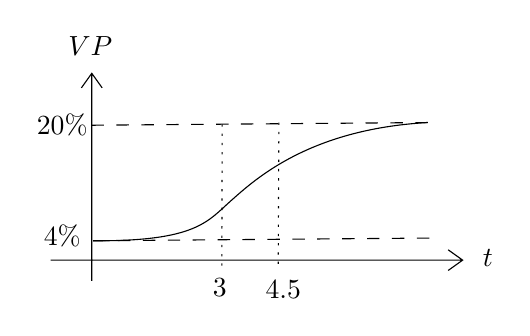
\begin{tikzpicture}[x=0.75pt,y=0.75pt,yscale=-1,xscale=1]
%uncomment if require: \path (0,300); %set diagram left start at 0, and has height of 300

%Shape: Axis 2D [id:dp8434144691544803] 
\draw  (171.87,196) -- (370.4,196)(191.72,106) -- (191.72,206) (363.4,191) -- (370.4,196) -- (363.4,201) (186.72,113) -- (191.72,106) -- (196.72,113)  ;
%Curve Lines [id:da3393494842698659] 
\draw    (192.33,186.67) .. controls (242.17,187) and (247.5,177.33) .. (258.83,167.33) .. controls (270.17,157.33) and (296.17,133) .. (353.17,129.73) ;


%Straight Lines [id:da6828905031101673] 
\draw  [dash pattern={on 4.5pt off 4.5pt}]  (191.6,131) -- (358,129.67) ;


%Straight Lines [id:da012395283086218845] 
\draw  [dash pattern={on 4.5pt off 4.5pt}]  (192.33,186.67) -- (358.73,185.33) ;


%Straight Lines [id:da9569907625895342] 
\draw  [dash pattern={on 0.84pt off 2.51pt}]  (281.87,129.73) -- (281.54,197.98) ;


%Straight Lines [id:da25982411660347404] 
\draw  [dash pattern={on 0.84pt off 2.51pt}]  (254.53,130.53) -- (254.39,200.06) ;


%%Straight Lines [id:da022260850258795317] 
%\draw    (160.2,170.6) -- (253.8,170.6) ;
%
%
%%Straight Lines [id:da5039184027623409] 
%\draw [line width=0.75]    (161,149.4) -- (282.6,149.4) ;



% Text Node
\draw (382.6,195.2) node   {$t$};
% Text Node
\draw (191,93) node   {$VP$};
% Text Node
\draw (177.5,131) node   {$20\%$};
% Text Node
\draw (177.5,184.5) node   {$4\%$};
% Text Node
\draw (253.4,209) node   {\SI{3}{\second}};
% Text Node
\draw (284,210) node   {\SI{4.5}{\second}};
%% Text Node
%\draw (135,145.5) node   {$0.632VP$};
%% Text Node
%\draw (135,168.5) node   {$0.283VP$};


\end{tikzpicture}

%	\centerline{\includegraphics[width=0.6\linewidth]{Figuras/Ch10/fig4.png}}
}

\frame{
	\frametitle{Lei de Faraday}
	\begin{block}{Introdução}
		Quando o fluxo magnético através da superfície de uma espira varia, surge na espira uma corrente elétrica induzida. Havendo corrente elétrica induzida no circuito, concluímos que deve haver uma \textbf{força eletromotriz induzida} que a originou.
		\begin{itemize}
			\item Experimentalmente, Faraday observou que, quanto mais rápida é a variação do fluxo magnético $\vec{\Phi}$, maior é a força eletromotriz induzida. Estabeleceu, então, que a \textbf{força eletromotriz induzida} ($\varepsilon$) \textbf{é proporcional à rapidez com que o fluxo magnético varia}. \\
		\end{itemize}
		$$\boxed{\vec{\varepsilon} = \dfrac{\Delta \vec{\Phi}}{\Delta t}}$$
	\end{block}
}

\frame{
	\frametitle{Lei de Faraday - Exemplo \#01}
	\begin{block}{}
		Uma espira plana de área $A = \SI{3.0e-3}{\meter\squared}$ está colocada paralelamente às linhas de indução de um campo magnético uniforme de intensidade $|\vec{B}| = \SI{8.0e-2}{\tesla}$. Gira-se a espira e, após um intervalo de tempo $\Delta t = \SI{0.40}{\second}$, a espira fica perpendicular às linhas de indução. Determine, nesse intervalo de tempo, o valor absoluto da fem.
	\end{block}
}

\frame{
	\frametitle{Lei de Faraday - Exemplo \#01}
	\begin{block}{Resolução}
		\begin{itemize}
			\item Para o instante $t = \SI{0}{\second}$: \\
			      \vspace{0.2cm}
			      $\vec{\Phi} = B \cdot A \cdot \cos \theta = B \cdot A \cdot \cos \ang{90} = \SI{0}{\weber}$
			\item Para o instante $t = \SI{0.4}{\second}$: \\
			      \vspace{0.2cm}
			      $\vec{\Phi} = B \cdot A \cdot \cos \theta = \num{8.0e-2} \cdot \num{3.0e-3} \cdot \cos\ang{0} = \SI{2.4e-4}{\weber}$
		\end{itemize}
		\vspace{0.4cm}
		Deste modo, $\vec{\varepsilon} = \dfrac{\Delta \vec{\Phi}}{\Delta t} = \dfrac{\num{2.4e-4} - 0}{\num{0.4} - 0} = \SI{6e-4}{\volt}$
	\end{block}
}

\frame{
	\frametitle{Lei de Lenz}
	\begin{block}{Introdução}
		Apesar de identificar que a corrente induzida variava de sentido, \textbf{Faraday não conseguiu determinar como ocorria essa variação}.
		\begin{itemize}
			\item Então em 1834, o físico russo Heinrich Lenz, propôs uma regra para a \textbf{definição do sentido da corrente induzida}.
		\end{itemize}
	\end{block}
}

\frame{
	\frametitle{Lei de Lenz}
	\begin{block}{A Lei}
		\textbf{``O sentido da corrente elétrica induzida é tal que seus efeitos (campo magnético produzido) se opõem à causa que lhe deu origem (variação do fluxo magnético que a produziu).''}
		\begin{itemize}
			\item Essa lei é representada na fórmula da força eletromotriz induzida através do \textbf{sinal de menos}.
			      $$\boxed{\vec{\varepsilon} = -\dfrac{\Delta \vec{\Phi}}{\Delta t}}$$
			\item Isso significa que \textbf{qualquer campo magnético produzido por uma corrente induzida será na direção oposta à variação do campo original}. Este resultado é frequentemente chamado de \textbf{Lei de Faraday-Lenz}.
		\end{itemize}
	\end{block}
}

\frame{
	\frametitle{Lei de Lenz}
	\begin{block}{A Lei}
		Em outras palavras: se o fluxo aumentou, a corrente vai querer que o fluxo diminua; se o fluxo diminuiu, a corrente vai querer que o fluxo aumente.
	\end{block}
	\centerline{\includegraphics[width=0.8\linewidth]{Figuras/Ch10/fig5.PNG}}
}

\frame{
	\frametitle{Lei de Lenz}
	\begin{block}{A Lei}
		Com essa afirmação pode-se concluir que quando um ímã é aproximado de uma espira, por exemplo, ele será repelido; e quando se afastar ele será atraído.
	\end{block}
	\centerline{\includegraphics[width=1\linewidth]{Figuras/Ch11/lenz.PNG}}
}

\frame{
	\frametitle{Transformadores}
	\begin{block}{Introdução}
		A energia elétrica após ser produzida nas usinas é transportada para os centros consumidores através de sistemas de transmissão. Contudo, antes de ser transportada para grandes distâncias, os dispositivos, chamados de \textbf{transformadores}, \textbf{elevam a tensão} para reduzir as perdas de energia. Quando essa energia chega até o seu destino final, \textbf{novamente ocorrerá a mudança no valor da tensão}.
		\begin{itemize}
			\item Assim, um \textbf{transformador é um dispositivo que serve para modificar uma tensão alternada, ou seja, aumenta ou diminui o seu valor de acordo com a necessidade}.
		\end{itemize}
	\end{block}
}

\frame{
	\frametitle{Transformadores}
	\begin{block}{Princípio de funcionamento}
		Um transformador é constituído por um núcleo de material ferromagnético no qual são enroladas \textbf{duas bobinas independentes}.
		\begin{itemize}
			\item A bobina conectada a fonte é chamada de \textbf{primário}, pois recebe a tensão que será transformada.
			\item A outra é chamada de \textbf{secundário}.
			\item Como a corrente que chega no primário é alternada, origina um \textbf{fluxo magnético} também alternado no núcleo do transformador. Essa variação do fluxo, gera uma \textbf{corrente alternada induzida no secundário}.
		\end{itemize}
	\end{block}
}

\frame{
	\frametitle{Transformadores}
	\begin{block}{Princípio de funcionamento}
		O aumento ou a diminuição da tensão induzida, \textbf{depende da relação entre o número de espiras nas duas bobinas}.
		\begin{itemize}
			\item Se o número de espiras no secundário for maior que no primário o transformador irá \textbf{elevar a tensão} e sendo ao contrário, ele irá \textbf{abaixar a tensão}.
		\end{itemize}
		$$\dfrac{V_p}{V_s} = \dfrac{N_p}{N_s}$$
	\end{block}
}

\frame{
	\frametitle{Transformadores}
	\centering
	\setmyunit{1cm}
	
	

\tikzset{every picture/.style={line width=0.75pt}} %set default line width to 0.75pt        

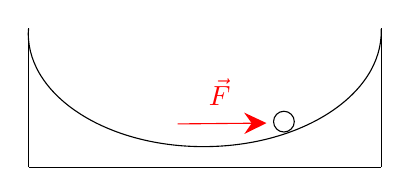
\begin{tikzpicture}[x=0.75pt,y=0.75pt,yscale=-1,xscale=1]
%uncomment if require: \path (0,300); %set diagram left start at 0, and has height of 300

%Straight Lines [id:da3398984480833569] 
\draw    (90,103) -- (90,170) ;


%Straight Lines [id:da39213437306955434] 
\draw    (260,103) -- (260,170) ;


%Straight Lines [id:da7536538469625644] 
\draw    (90,170) -- (260,170) ;


%Shape: Arc [id:dp6883804097522237] 
\draw  [draw opacity=0] (260,103) .. controls (260,103) and (259.87,104.01) .. (259.88,104.37) .. controls (260.12,134.75) and (222.24,159.67) .. (175.28,160.04) .. controls (128.31,160.41) and (90.05,136.08) .. (89.81,105.71) .. controls (89.81,105.53) and (89.81,105.35) .. (89.81,105.17) -- (174.84,105.04) -- cycle ; \draw   (259.85,103.29) .. controls (259.87,103.65) and (259.87,104.01) .. (259.88,104.37) .. controls (260.12,134.75) and (222.24,159.67) .. (175.28,160.04) .. controls (128.31,160.41) and (90.05,136.08) .. (89.81,105.71) .. controls (89.81,105.53) and (90,103) .. (90,103) ;
%Shape: Circle [id:dp54266808828771] 
\draw   (208,148) .. controls (208,145.24) and (210.24,143) .. (213,143) .. controls (215.76,143) and (218,145.24) .. (218,148) .. controls (218,150.76) and (215.76,153) .. (213,153) .. controls (210.24,153) and (208,150.76) .. (208,148) -- cycle ;
%Straight Lines [id:da8066991195909812] 
\draw [color={rgb, 255:red, 255; green, 0; blue, 0 }  ,draw opacity=1 ]   (161.8,149.1) -- (202.6,148.72) ;
\draw [shift={(204.6,148.7)}, rotate = 539.46] [fill={rgb, 255:red, 255; green, 0; blue, 0 }  ,fill opacity=1 ][line width=0.75]  [draw opacity=0] (10.72,-5.15) -- (0,0) -- (10.72,5.15) -- (7.12,0) -- cycle    ;


% Text Node
\draw (120,147) node  [align=left] {};
% Text Node
\draw (182,133.8) node [color={rgb, 255:red, 255; green, 0; blue, 0 }  ,opacity=1 ]  {$\vec{F}$};


\end{tikzpicture}

	
%	\centerline{\includegraphics[width=0.9\linewidth]{Figuras/Ch10/fig6.jpg}}
}

\section*{Exercícios}
\frame{
	\frametitle{Exercícios}
	\begin{block}{}
		01. A corrente elétrica no enrolamento primário de um transformador corresponde a \SI{10}{\ampere}, enquanto no enrolamento secundário corresponde a \SI{20}{\ampere}.
		Sabendo que o enrolamento primário possui 1200 espiras, determine o número de espiras do enrolamento secundário.

		\vspace{0.5cm}

		02. Uma espira circular de raio \SI{0.2}{\meter} está sob influência de um campo magnético de módulo \SI{5}{\tesla}. Determine o fluxo magnético sobre a espira considerando que o ângulo entre o vetor campo magnético e a reta normal ao plano dessa espira seja de $\ang{60}$.
	\end{block}
}

\section*{Referências}
\frame{
	\frametitle{Referências e Exercícios Complementares}
	\begin{itemize}
		\item ALEXANDRE, Charles K.; SADIKU, Matthew N. O. Fundamentos de Circuitos Elétricos. 5. ed. Porto Alegre: AMGH, 2013.
	\end{itemize}
	%\centering{\alert{Página 36 - \textbf{1.6.1 até 1.6.5, 1.6.17 até 1.6.19}}} \\
	\centering{\alert{Lista de exercícios 10}}
}